\section{Computational Complexity of Real Functions}
\label{section: preliminaries}

\subsection{Computation of Real Function}

Real numbers are represented by functions from string to string.
\begin{definition}
 A function $\phi \colon \{0\} ^* \to \{0, 1\}^*$ is a \emph{name} of a real number $x$ 
 if for all $n \in \N$,
  $\phi(0^n)$ is the binary representation of $\lfloor x \cdot 2^n \rfloor$ or
  $\lceil x \cdot 2^n \rceil$,
 where $\lfloor \cdot \rfloor$ and $\lceil \cdot \rceil$ are 
 rounding down and up functions.
 \end{definition}
In effect, a name of a real number $x$ receive $n$ and return approximation of $x$ with precision $2^{-n}$.

We use \emph{oracle Turing machines}(henceforth just machines)
to work on names of real numbers(Figure \ref{fig:model-of-function}).

 \begin{figure}
  \begin{center}
   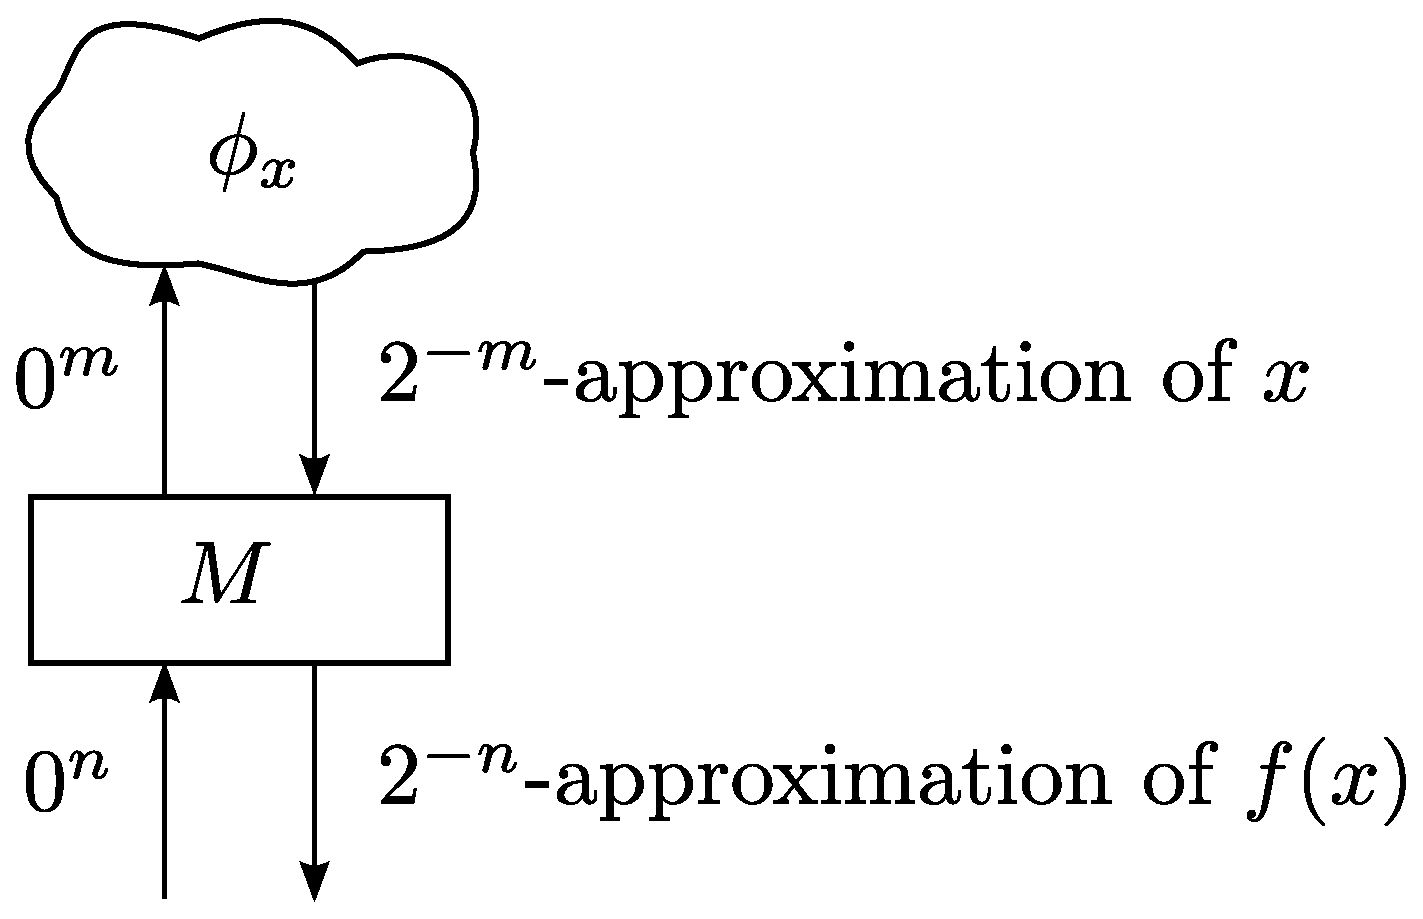
\includegraphics[height=0.15\textheight]{image/model-of-function.eps}
  \end{center}
  \caption{A machine $M$ computing a real function $f$}
  \label{fig:model-of-function}
 \end{figure}

Let $M$ be a machine and $\phi$ be a function from string to string,
We write $M ^\phi (0 ^n)$ as the output string by computation of $M$ given
$\phi$ as oracle and string $0^n$ as input.
So we also regard $M^\phi$ as a function from string to string.

\begin{definition}
Let $A$ be a bounded closed interval of $\R$.
A machine $M$ \emph{computes} a real function $f \colon A \to \R$ 
if for any $x \in A$ and any name $\phi_x$ of it,
$M^{\phi_x}$ is a name of $f(x)$.
\end{definition}

When $A$ is a bounded closed interval of $\R ^2$,
we define a machine computing $f \colon A \to \R$ in a similar way using machines with two oracles.
A real function is (\emph{polynomial-time}) \emph{computable} if there exists some machine that computes it (in polynomial time).

When a machine $M$ computes a real function $f$,
for each demanded precision $2^{-n}$,
 precision $2^{-m}$.
Computable real functions are continuous.
Giving all approximations of functions at rational points an relation between $n$ and $m$,
we can characterize (polynomial-time) computability of real function
without oracle Turing machines

\begin{lemma}
 \label{lem:type1representation}
 A real function is (polynomial-time) computable if and only if
 there exist a (polynomial-time) computable function 
 $\phi \colon (\Q \cap [0, 1]) \times \{0\} ^* \to \Q$ and 
 polynomial $p \colon \N \to \N$ such that
 for all $d \in \Q \cap [0,1]$ and $n \in \N$,
 \begin{equation}
  |\phi(d, 0^n) - f(d)| \le 2^{-n},
 \end{equation}
 and for all $x, y \in [0, 1]$, $m \in \N$,
 \begin{equation}
  |x-y| \le 2^{-p(m)} \Rightarrow |f(x) - f(y)| \le 2^{-m}.
 \end{equation}
 where each rational number in $\Q$ is represented by a pair of integers in binary representation.
\end{lemma}

\subsection{Reduction and Hardness}
A language $L \subseteq \{0, 1\} ^*$ is identified with the function
$L \colon \{0, 1\} ^* \to \{0, 1\}$ such that $L (u) = 1$ if and only if $u \in L$.

\begin{definition}[Reduction]
 A Language $L$ reduces to a real function $f \colon [0, 1] \to \R$
 if there exists a polynomial-time function $S$ and a polynomial-time oracle Turing machine $M$ (Figure \ref{fig:reduction})
 such that for any string $u$:
 \begin{figure}
  \begin{center}
  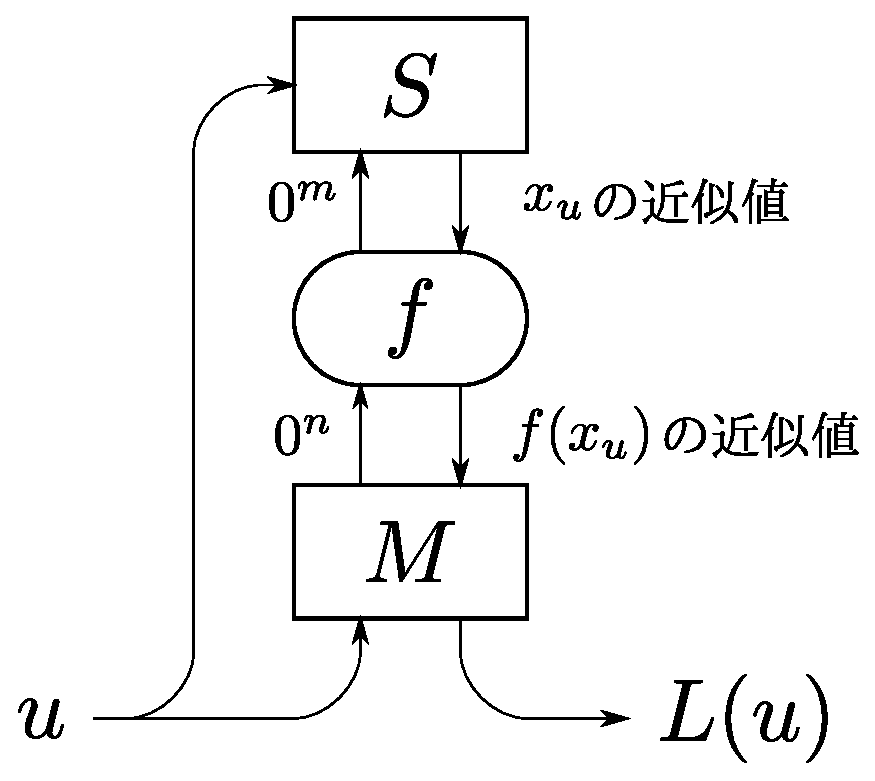
\includegraphics[scale=0.25]{image/reduction.eps}
  \caption{Reduction from a language $L$ to a function $f \colon [0,1] \to \R$}
  \label{fig:reduction}
  \end{center}
 \end{figure}
  \begin{enumerate}
   \item $S(u, \cdot)$ is a name of $x_u$;
   \item $M^\phi(u)$ accepts if and only if $u \in L$ for any name $\phi$ of $f(x_u)$.
  \end{enumerate}
\end{definition}
As a matter of form this definition is different from 
that by Kawamura but they have same power as reduction.
Let $C$ be a complexity class, a function $f$ is \emph{$C$-hard}
if for all language in $C$ is reducible to $f$.
